\chapter*{直线和圆}
\subsection*{直线方程}
\begin{enumerate}
    \item 若直线 $l$ 的斜率 $k \in \left( -1,\sqrt{3}\right)$ ，则直线 $l$ 的倾斜角的取值范围是\blkda[3]{$\left[0, \dfrac{\pi}{3}\right) \cup \left(\dfrac{3\pi}{4}, \pi\right)$}.
    \item 已知点 $A(4,2)$ ， $B(0,3)$ 和直线 $l$ : $mx - y - 3m + 1 = 0$ ( $m \in \mathbf{R}$ )，直线 $l$ 与线段 $AB$ 有公共点，则 $m$ 的取值范围是\blkda[3]{$\left(-\infty, -\dfrac{2}{3}\right]\cup \left[1, +\infty\right)$}.
    \item 过点 $A(3,6)$ 的直线在两坐标轴上的截距之和为零，则该直线方程为\blkda[3]{$y = 2x$或$y = x+3$}.
    \item 已知直线 $l_1 : ax + y + 1 = 0$ 与直线 $l_2 : (a - 1) x - ay + 2 = 0$ 垂直，则实数 $a$ 的值为\blkda{2或0}.
    \item 已知直线 $l_1 : mx + 2y - 2 = 0$ 与直线 $l_2 : 5x + (m + 3) y - 5 = 0$ ，若 $l_1//l_2$ ，则 $m =$ \blkda{$-5$}
    \item 在平面直角坐标系中， $\bigtriangleup ABC$ 的三个顶点分别为 $A(-1, - 3)$ 、 $B(1,1)$ 、 $C(4,2)$ .
    \begin{enumerate}
        \item 求 $AC$ 边的高线 $l_1$ 的直线方程
        \item 求 $AB$ 边的垂直平分线 $l_2$ 的直线方程
        \item 求 $\bigtriangleup ABC$ 的外接圆的一般方程
    \end{enumerate}
    \begin{jieda}
        \begin{enumerate*}
            \item $x+y-2=0$
            \item $x+2y+2=0$
            \item $x^2+y^2-8x+6y=0$
        \end{enumerate*}
    \end{jieda}
    \item 已知三角形 $ABC$ 的顶点 $C(1,3)$ ,边 $AC$ 上的高 $BH$ 所在的直线方程为 $2x - y - 3 = 0$ ,边 $AB$ 的中点为 $D\left( -\dfrac{1}{2},3\right)$.
    \begin{enumerate}
        \item 求边 $AC$ 所在直线的方程
        \item 求点 $B$ 的坐标
        \item 求 $\angle BCA$ 的平分线所在直线的方程
    \end{enumerate}
    \begin{jieda}
        \begin{enumerate*}
            \item $x+2y-7 = 0$
            \item $(2,1)$
            \item $x-y+2=0$
        \end{enumerate*}
    \end{jieda}
\end{enumerate}
\subsection*{夹角}
\begin{enumerate}
    \item 直线 $2x - 3y + 1 = 0$ 与 $x + 5y - 10 = 0$ 的夹角为\blkda{$\dfrac{\pi}{4}$}.
    \item 已知直线 $2x - ay - 4 = 0$ 与直线 $2x + y + 1 = 0$ 的夹角为 $\arccos \dfrac{2\sqrt{5}}{5}$ ,则实数 $a =$\blkda{$-\dfrac{8}{3}$或$0$}
    \item 若直线 $x = my + 3$ 与直线 $x - \sqrt{3}y = 0$ 的夹角是 $\dfrac{\pi}{6}$ ,则实数 $m$ 的值是\blkda{$\dfrac{\sqrt{3}}{3}$}.
    \item 若直线 $l_1 : \left( \sqrt{2} + 1\right) ax - y + a = 0,l_2 : ax - \left( \sqrt{2} + 1\right) y - a = 0$ ,其中 $a \neq 0$ ,则 $l_1$ 与 $l_2$ 夹角的取值范围为\blkda{$\left(0, \dfrac{\pi}{4}\right]$}.
\end{enumerate}
\subsection*{距离}
\begin{enumerate}
    \item $l_1 : x - y + 3 = 0$ 与直线 $l_2 : 2x + my - 2 = 0$ 平行，则直线 $l_1$ 与 $l_2$ 的距离为\blkda{$2\sqrt{2}$}.
    \item 点 $A(1,0) ,B(3,0)$ 到直线 $l$ 的距离都等于 1,直线 $l$ 的条数是\blkda{3}.
    \item 若直线 $l$ 过点 $P(-1,2)$ 且到点 $A(2,3)$ 和点 $B(-4,5)$ 的距离相等，则直线 $l$ 的方程为\blkda[4]{$x+3y-5=0$或$x=-1$}.
\end{enumerate}
\subsection*{对称}
\begin{enumerate}
    \item 若点 $M(1,1)$ 与点 $N(5, - 1)$ 关于直线 $l$ 对称，则直线 $l$ 的一般式方程为\blkda[3]{$2x-y-6=0$}.
    \item 直线 $x + y = 0$ 关于点 $(1,1)$ 对称的直线方程是\blkda[3]{$x+y-4=0$}.
    \item 直线 $l_1 : 3x - y - 3 = 0$ 关于直线 $l_2 : x + y - 1 = 0$ 的对称直线方程为\blkda[3]{$x-3y-1=0$}.
\end{enumerate}
\subsection*{直线其他}
\begin{enumerate}
    \item 已知两直线 $l_1 : x - 2y + 4 = 0,l_2 : 4x + 3y + 5 = 0$ . 若直线 $l_3 : ax + 2y - 6 = 0$ 与 $l_1,l_2$ 不能构成三角形,求实数 $a =$\blkda[3]{$-1$或$-2$或$\dfrac{8}{3}$}
    \item 设 $m \in \mathbf{R}$ ,过定点 $A$ 的动直线 $x + 1 + my = 0$ 和过定点 $B$ 的动直线 $mx - y - m + 3 = 0$ 交于点 $P(x,y)$ ,则 $\sqrt{3}|PA| + |PB|$ 的最大值是\blkda{$2\sqrt{13}$}.
\end{enumerate}
\subsection*{圆的方程}
\begin{enumerate}
    \item 设点 $M$ 在直线 $2x + y - 1 = 0$ 上，点 $(3,0)$ 和 $(0,1)$ 均在 $\odot M$ 上，则 $\odot M$ 的方程为\blkda[4]{$(x-1)^2+(y+1)^2 = 5$}.
    \item 若点 $P(1,2)$ 在圆 $x^2 + y^2 - x + y + k = 0$ 外，则实数 $k$ 的取值范围为\blkda{$\left(-6, \dfrac{1}{2}\right)$}.
    \item 对任意实数 $m$ ，圆 $x^2 + y^2 - 3mx - 6my + 9m - 2 = 0$ 恒过定点，则定点坐标为\blkda[3]{$(1, 1), \left(\dfrac{1}{5}, \dfrac{7}{5}\right)$}.
\end{enumerate}
\subsection*{垂径定理}
\begin{enumerate}
    \item 若直线 $x - y + m = 0(m > 0)$ 被圆 $\left( x - 1\right)^2 + \left( y - 1\right)^2 = 3$ 截得的弦长为 $m$ ,则 $m$ 的值为\blkda{2}.
    \item 在平面直角坐标系 $xOy$ 中,直线 $l : mx + y - m = 0$ 被圆 $M : x^2 + y^2 - 4x - 2y + 1 = 0$ 截得的最短弦的长度为\blkda{$2\sqrt{2}$}.
\end{enumerate}
\subsection*{极点极线}
\begin{enumerate}
    \item 已知直线 $l : {ax} + {by} - {r}^{2} = 0$ 与圆 $C : {x}^{2} + {y}^{2} = {r}^{2}$ ,点 $A\left( {a,b}\right)$ ,则下列说法正确的有\blkda{\ding{172}\ding{173}\ding{175}}
    \begin{dingautolist}{172}
        \item 若点 $A$ 在圆 $C$ 上,则直线 $l$ 与圆 $C$ 相切
        \item 若点 $A$ 在圆 $C$ 内,则直线 $l$ 与圆 $C$ 相离
        \item 若点 $A$ 在圆 $C$ 外,则直线 $l$ 与圆 $C$ 相离
        \item 若点 $A$ 在直线 $l$ 上,则直线 $l$ 与圆 $C$ 相切
    \end{dingautolist}
    \begin{jieda}
        圆心 $C\left( {0,0}\right)$ 到直线 $l$ 的距离 $d = \dfrac{{r}^{2}}{\sqrt{{a}^{2} + {b}^{2}}}$
        \begin{dingautolist}{172}
            \item 
            
            若点 $A\left( {a,b}\right)$ 在圆 $C$ 上,则 ${a}^{2} + {b}^{2} = {r}^{2}$，所以 $d = \dfrac{{r}^{2}}{\sqrt{{a}^{2} + {b}^{2}}} = \left| r\right|$，则直线 $l$ 与圆 $C$ 相切
            \item 若点 $A\left( {a,b}\right)$ 在圆 $C$ 内,则 ${a}^{2} + {b}^{2} < {r}^{2}$，所以 $d = \dfrac{{r}^{2}}{\sqrt{{a}^{2} + {b}^{2}}} > \left| r\right|$，则直线 $l$ 与圆 $C$ 相离

            \item 若点 $A\left( {a,b}\right)$ 在圆 $C$ 外,则 ${a}^{2} + {b}^{2} > {r}^{2}$，所以 $d = \dfrac{{r}^{2}}{\sqrt{{a}^{2} + {b}^{2}}} < \left| r\right|$ ,则直线 $l$ 与圆 $C$ 相交        
            \item 若点 $A\left( {a,b}\right)$ 在直线 $l$ 上,则 ${a}^{2} + {b}^{2} - {r}^{2} = 0$，即 ${a}^{2} + {b}^{2} = {r}^{2}$，所以 $d = \dfrac{{r}^{2}}{\sqrt{{a}^{2} + {b}^{2}}} = \left| r\right|$，则直线 $l$ 与圆 $C$ 相切
        \end{dingautolist}
    \end{jieda}
    \item 若点 $P(a_1,b_1) ,Q(a_2,b_2)$ 的坐标满足 $\left\{ \begin{array}{l} 
        a_1\cos \theta + b_1\sin \theta = 3 \\  
        a_2\cos \theta + b_2\sin \theta = 3 
    \end{array} \right.$，则点 $M\left( \sqrt{3}, -1\right)$ 到直线 $PQ$ 的距离的最大值为\blkda{5}
\end{enumerate}
\subsection*{直线和圆相切}
\begin{enumerate}
    \item 若直线 $kx - y - 2k + 3 = 0$ 与圆 $x^2 + \left( y + 1\right)^2 = 4$ 相切,则 $k =$ \blkda{$\dfrac{3}{4}$}.
    \item 过点 $(4,4)$ 与圆 $x^2 + y^2 - 4x = 0$ 相切的直线方程为\blkda[4]{$x = 4$或$3x-4y+4=0$}.
    \item 过点 $P(1,3)$ 作圆 $C : \left( x - 2\right)^2 + y^2 = 10$ 的切线，则切线方程为\blkda[3]{$x-3y+8=0$}.
    \item 过点 $P(4, - 1)$ 作圆 $C : x^2 + y^2 + 2x - 4y - 4 = 0$ 的切线，切点为 $A$ 、 $B$ ，则过切点 $A$ ， $B$ 的直线方程为\blkda[3]{$5x-3y+2=0$}.
    \item 由直线 $y = x + 1$ 上任一点 $P$ 向圆 $C\left( x + 3\right)^2 + y^2 = 1$ 引切线，切点为 $A$ ， $B$ ，则四边形 $PACB$ 面积的最小值为\blkda{1}.
    \item 已知圆 $O : x^2 + y^2 = 1$ 与 $x$ 轴负半轴的交点为 $A,P$ 为直线 $3x + 4y - a = 0$ 上一点,过 $P$ 作圆 $O$ 的切线, 切点为 $T$ ，若 $PA = 2PT$ ，则 $a$ 的最大值为\blkda{$\dfrac{23}{3}$}.
    \item 已知 $A(2,0) ,B(10,0)$ ，若直线 $tx - 4y + 2 = 0$ 上存在点 $P$ ，使得 $\vv{PA} \cdot \vv{PB} = 0$ ，则 $t$ 的取值范围为\blkda{$\left[-\dfrac{21}{5}, 3\right]$}.
\end{enumerate}
\subsection*{求代数式范围}
\begin{enumerate}
    \item 已知实数 $x,y$ 满足 $x^2 + y^2 - 2x + 4y - 20 = 0$ . 求:
    \begin{enumerate}
        \item $x^2 + y^2$ 的取值范围
        \item $\dfrac{y - 4}{x - 6}$ 的取值范围
        \item $x - 2y$ 的取值范围
    \end{enumerate}
    \begin{jieda}
        \begin{enumerate*}
            \item $\left\lbrack 30 - 10\sqrt{5},30 + 10\sqrt{5}\right\rbrack$
            \item $\left\lbrack \dfrac{11}{60}, + \infty \right) $
            \item $ \left\lbrack 5 - 5\sqrt{5},5 + 5\sqrt{5}\right\rbrack$
        \end{enumerate*}
    \end{jieda}
\end{enumerate}
\subsection*{圆与圆的位置关系}
\begin{enumerate}
    \item 已知 $\odot C_1 : \left( x + 1\right)^2 + \left( y + \dfrac{3}{2}\right)^2 = \dfrac{9}{4}$ 与 $\odot C_2 : x^2 + y^2 + 4x + 3y + m = 0$ 有且只有两条公切线,则实数 $m$ 的取值范围是\blkda{$(0, 6)$}.
    \item 圆 ${C}_{1} : {x}^{2} + {y}^{2} - {2x} + {10y} - {24} = 0$ 与圆 ${C}_{2} : {x}^{2} + {y}^{2} + {2x} + {2y} - 8 = 0$ 的公共弦所在直线的方程为\blkda[3]{$x - {2y} + 4 = 0$},公共弦长为\blkda{$2\sqrt{5}$}.
    \begin{jieda}
        联立两圆的方程得 $\left\{  \begin{array}{l} {x}^{2} + {y}^{2} - {2x} + {10y} - {24} = 0 \\  {x}^{2} + {y}^{2} + {2x} + {2y} - 8 = 0, \end{array}\right.$
        
        两式相减并化简,得 $x - {2y} + 4 = 0$，即为两圆公共弦所在直线的方程.
        
        由 ${x}^{2} + {y}^{2} - {2x} + {10y} - {24} = 0$ ,
        
        得 ${\left( x - 1\right) }^{2} + {\left( y + 5\right) }^{2} = {50}$，故圆 ${C}_{1}$ 的圆心坐标为$(1, -5)$,半径 $r = 5\sqrt{2}$ ,
        
        圆心到直线 $x - {2y} + 4 = 0$ 的距离为 $d = \dfrac{\left| 1 - 2 \times  \left( -5\right)  + 4\right| }{\sqrt{1 + {\left( -2\right) }^{2}}} = 3\sqrt{5}$ .
        
        故公共弦长$l = 2\sqrt{r^2-d^2} = 2\sqrt{5}$ .
    \end{jieda}
\end{enumerate}
\subsection*{阿氏圆调整系数}
\begin{enumerate}
    \item 在平面直角坐标系 $xOy$ 中,点 $A(4,0) ,B(1,0) ,C(-1,0) ,D(0,1)$ ,若点 $P$ 满足 $|PA| = 2|PB|$ ,则 $|PC| + \dfrac{1}{2}|PD|$ 的最小值为\blkda{$\dfrac{\sqrt{17}}{2}$}
    \item 已知椭圆 $\dfrac{{x}^{2}}{6} + \dfrac{{y}^{2}}{2} = 1$ 的右焦点为 $F$ ,上顶点为 $A$ ,点 $P$ 在圆 ${x}^{2} + {y}^{2} = 8$ 上,点 $Q$ 在椭圆上,则 $2\left| {PA}\right|  + \left| {PQ}\right|  - \left| {QF}\right|$ 的最小值是\blkda{$6-2\sqrt{6}$}.
    \begin{jieda}
        设左焦点为$F_1$，根据椭圆的定义可知$2\left| {PA}\right|  + \left| {PQ}\right|  - \left| {QF}\right| = 2\left| {PA}\right|  + \left| {PQ}\right|  + \left| {QF_1}\right| - 2a \geq 2|PA| + |PF_1| - 2\sqrt{6}$

        
        \begin{dingautolist}{172}
            \item 法1

            设$2|PA| = |PM|$，$M(a, b)$，则$2\sqrt{x^{2} + (y-\sqrt{2})^{2}} = \sqrt{(x-a)^2+(y-b)^2}$，两侧平方整理有$3x^2+2ax-a^2+3y^2+(2b-8\sqrt{2})y+8-b^2 = 0$为$P$的轨迹方程，故与$x^2+y^2 = 8$比较系数可得$\left\{\begin{array}{l}
                    a = 0 \\
                    b = 4\sqrt{2}
            \end{array}\right.$，因此$M(0, 4\sqrt{2})$
        
            \item 法2
            
            $\left| {PA}\right|  = \sqrt{x^{2} + (y-\sqrt{2})^{2}} = \dfrac{1}{2}\sqrt{4{x}^{2} + 4{y}^{2} - 8\sqrt{2}y + 8} = \dfrac{1}{2}\sqrt{{x}^{2} + {y}^{2} -8\sqrt{2}y + 32} = \dfrac{1}{2}\sqrt{x^2 + (y-4\sqrt{2})^{2}}$ 
            
            设 $M(0, 4\sqrt{2})$ ,则 $\left| {PA}\right|  = \dfrac{1}{2}\left| {PM}\right|$
        \end{dingautolist}

        故$2|PA| + |PF_1| - 2\sqrt{6} = |PM| + |PF_1| - 2\sqrt{6} \geq |MF_1| - 2\sqrt{6} = 6-2\sqrt{6}$
    \end{jieda}
\end{enumerate}
\subsection*{平面向量与圆}
\begin{enumerate}
    \item 若向量$\vv{a} = (1, 1), \vv{b} = (1, -1), \vv{c} = (\sqrt{2} cos\alpha, \sqrt{2}sin\alpha) (\alpha \in \mathbf{R})$，实数$m, n$满足$m \vv{a} + n \vv{b} = \vv{c}$，则$(m-3)^2+n^2$的取值范围是\blkda{$[4, 16]$}
    \begin{jieda}
        $\left \{ \begin{array}{l}
                m+n = \sqrt{2}cos\alpha  \\
                m-n = \sqrt{2}sin\alpha
        \end{array} \right.$，平方相加即得$m^2+n^2 = 1$，因此，点$(m,n)$在单位圆上，$(m-3)^2+n^2$为点$(m,n)$到$(3,0)$的距离平方，根据几何关系可知其取值范围是$[4, 16]$
    \end{jieda}
    
    \item 已知向量$\vv{a}, \vv{b}, \vv{c}$满足$|\vv{a}| = 2, |\vv{b}| = 3, \vv{a} \cdot \vv{b} = 3, |\vv{c}|^2 - 2\vv{b} \cdot \vv{c} + 8 = 0$，若$\vv{c} = \lambda \vv{a} + (1-\lambda) \vv{b}$，则$\lambda$的值为\blkda{$\pm \dfrac{\sqrt{7}}{7}$}
    \begin{jieda}
        根据条件可知$\vv{a}, \vv{b}$夹角为$\dfrac{\pi}{3}$，以$\vv{b}$的方向为$x$轴正方向，设$B(3, 0), A(1, \sqrt{3})$即$\vv{OA} = \vv{a}, \vv{OB} = \vv{b}$，建立平面直角坐标系。根据等和线结论可知$\vv{OC} = \vv{c}$的终点$C$在直线$AB: y = -\dfrac{\sqrt{3}}{2}(x-3)$上.
        
        设$C(x, y)$，所以$|\vv{c}|^2 - 2\vv{b} \cdot \vv{c} + 8 = 0$可以转化为$x^2+y^2 - 6x + 8 = 0$，故$C$在以$B$为圆心，1为半径的圆上.
        
        $\vv{OC} = \vv{OB} + \vv{BC} = \vv{OB} \pm \dfrac{\sqrt{7}}{7}\vv{BA}$，即$\vv{c} = \vv{b} \pm \dfrac{\sqrt{7}}{7}(\vv{a} - \vv{b})$，故$\lambda = \pm \dfrac{\sqrt{7}}{7}$
    \end{jieda}

    \item 已知平面向量满足$|\vv{a}| = |\vv{b}| = \vv{a} \cdot \vv{b} = \vv{c} \cdot (\vv{a} + 2\vv{b}-2\vv{c}) = 2$，若$|\vv{a} - \vv{c}|$的最大值、最小值分别为$M, N$，则$\dfrac{M}{N} = $\blkda{$\dfrac{5+\sqrt{21}}{2}$}
    \begin{jieda}
        以$\vv{a}$为$x$轴正方向建立平面直角坐标系，故设$\vv{a} = (2, 0), \vv{b} = (1, \sqrt{3}), \vv{c} = (x, y)$，故$\vv{c} \cdot (\vv{a} + 2\vv{b}-2\vv{c}) = 2$即$x \cdot (4-2x) + y \cdot (2\sqrt{3} - 2y) = 2$，化简配方可得$(x-1)^2 + (y - \dfrac{\sqrt{3}}{2})^2 = \dfrac{3}{4}$，故$\vv{c}$的终点位于圆心为$(1, \dfrac{\sqrt{3}}{2})$，半径为$\dfrac{\sqrt{3}}{2}$的圆上，故根据几何关系可知$\dfrac{\sqrt{7} - \sqrt{3}}{2} \leq |\vv{a} - \vv{c}| \leq \dfrac{\sqrt{7} + \sqrt{3}}{2}$，即$M = \dfrac{\sqrt{7}+\sqrt{3}}{2}, N = \dfrac{\sqrt{7} - \sqrt{3}}{2}$，故$\dfrac{M}{N} = \dfrac{5+\sqrt{21}}{2}$
    \end{jieda}
    
    \item 已知圆$O$的半径为1，直线$PA$与圆$O$相切于点$A$，直线$PB$与圆$O$交于$B$，$C$两点，$D$为$BC$的中点，若$|PO| = \sqrt{2}$，则$\vv{PA} \cdot \vv{PD}$的最大值为\blkda{$\dfrac{1+\sqrt{2}}{2}$}
    \begin{jieda}
        以$A$为原点建系，设圆$O:x^2+(y-1)^2 = 1$，$P(1, 0)$

        根据过定点的弦的中点轨迹的性质可知$D$在圆$x^2 + y^2 - x - y = 0$上（利用点差法/$\angle ODP = \ang{90}$的性质均可求），故设$D\left(\dfrac{1}{2}+\dfrac{\sqrt{2}}{2}cos\theta, \dfrac{1}{2}+\dfrac{\sqrt{2}}{2}sin\theta\right), \theta \in \left(\dfrac{3\pi}{4}, \dfrac{5\pi}{4}\right)$
        
        故$\vv{PA} = (-1, 0), \vv{PD} = \left(-\dfrac{1}{2}+\dfrac{\sqrt{2}}{2}cos\theta, \dfrac{1}{2}+\dfrac{\sqrt{2}}{2}sin\theta\right)$，故$\vv{PA}  \cdot \vv{PD} = \dfrac{1}{2}-\dfrac{\sqrt{2}}{2}cos\theta \in \left(0, \dfrac{1+\sqrt{2}}{2}\right]$.
    \end{jieda}

    \item 在平面上，$\vv{AB_1} \perp \vv{AB_2}, |\vv{OB_1}| = |\vv{OB_2}| = 1$，$\vv{AP} = \vv{AB_1} + \vv{AB_2}$，若$|\vv{OP}| < \dfrac{1}{2}$，则$|\vv{OA}|$的取值范围是\blkda{$\left(\dfrac{\sqrt{7}}{2}, \sqrt{2}\right]$}
    \begin{jieda}
        设$A(a, 0)$，方法同上，可得$P$的方程为$x^2+y^2 = 2-a^2$，因此$2-a^2 \in \left[0, \dfrac{1}{4}\right)$，故$a \in \left(\dfrac{\sqrt{7}}{2}, \sqrt{2}\right]$
    \end{jieda}
\end{enumerate}
\subsection*{矩形的顶点在同心圆上}
\begin{enumerate}
    \item 已知圆$O$的半径为2，$P$是圆内一定点，$|OP| = 1$，$A, B$为圆$O$上两个动点满足$PA \perp PB$，存在$C$使得$PACD$为矩形，则$\vv{OC} \cdot \vv{OP}$的取值范围是\blkda[2]{$[-\sqrt{7}, \sqrt{7}]$}
    \begin{jieda}
        如图，连接 ${AB}$ ,设 ${AB}$ 与 ${CP}$ 交于点 $M,C\left( {x,y}\right)$ ,不妨设 $P\left( {1,0}\right)$
        \begin{center}
            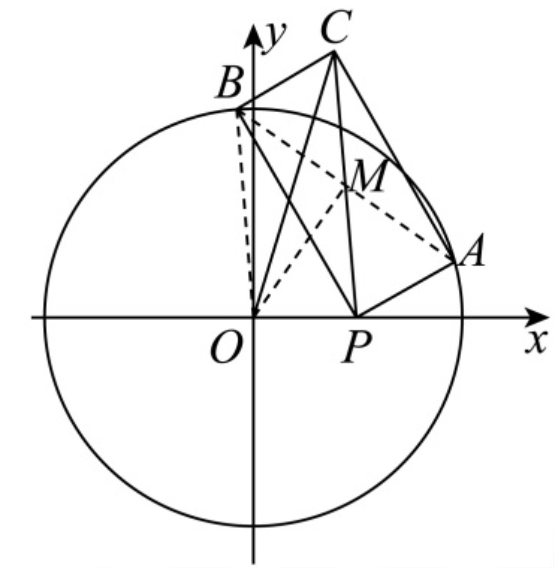
\includegraphics[width=0.2\textwidth]{bodyxb/src/juxing1.png}
        \end{center}
        因为 $\vv{PA} \cdot  \vv{PB} = 0,\vv{PC} = \vv{PA} + \vv{PB}$，所以四边形 ${PACB}$ 是矩形,则 $M\left( {\dfrac{x + 1}{2},\dfrac{y}{2}}\right) ,{PM} = {MB}$ .
        连接 ${OM},{OB}$ ,在 ${Rt\Delta OBM}$ 中, ${OM} \bot  {BM}$，所以 $O{B}^{2} = O{M}^{2} + B{M}^{2} = O{M}^{2} + M{P}^{2}$，即$4 = {\left( \dfrac{x + 1}{2}\right) }^{2} + {\left( \dfrac{y}{2}\right) }^{2} + {\left( \dfrac{x + 1}{2} - 1\right) }^{2} + {\left( \dfrac{y}{2}\right) }^{2}$ ,即 ${x^2} + {y^2} = 7$ ,
        所以 $x \in  \left\lbrack  {-\sqrt{7},\sqrt{7}}\right\rbrack$ ,所以 $\vv{OC} \cdot  \vv{OP} = x \in  \left\lbrack  {-\sqrt{7},\sqrt{7}}\right\rbrack$ .
        故$\vv{OC} \cdot \vv{OP}$的取值范围是$[-\sqrt{7}, \sqrt{7}]$
    \end{jieda}
    \item (2025$\cdot$普陀区一模$\cdot$10)设平面上四点 $P$ 、 $Q$ 、 $M$ 、 $N$ 满足: $\left| {PM}\right|  = \left| {PN}\right|  = 4$ ， $\left| {PQ}\right|  = 2$ ，若 $\vv{QM} \cdot  \vv{QN} = 0$ ，则 $\left| {MN}\right|$ 的最小值为\blkda[2]{$2\sqrt{7} - 2$}.
    \begin{jieda}
        以$P$为原点，$\vv{PQ}$为$x$轴正方向建系，$Q(2, 0)$，$M,N$在以$P$为圆心，$4$为半径的圆上，根据垂径定理可知$P$到$MN$距离越大，$|MN|$越小.
        
        取 ${MN}$ 的中点 $F$，则$|PF|$为$P$到$MN$距离，根据几何关系应满足$|PF| \leq |PQ| + |QF|$，设$|MN| = 2t, t > 0$，则$|PF| = \sqrt{16-t^2}$，$|QF| = \dfrac{|MN|}{2} = t$，因此$\sqrt{16-t^2} \leq 2+t$，解得$t \geq \sqrt{7}-1$，故$\left| {MN}\right|$ 的最小值为 $2\sqrt{7}-2$.
        \begin{center}
        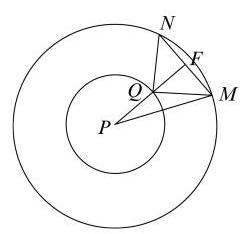
\includegraphics[width=0.2\textwidth]{bodyxb/src/97_576_1182_244_234_0.jpg}
        \end{center}

        \ps $|PF|$变大$\Longleftrightarrow |QF|$变小，在三点共线时取得最值.
    \end{jieda}
    \item (2024$\cdot$长宁区二模$\cdot$12)已知平面向量 $\vv{a}$ 、 $\vv{b}$ 、 $\vv{c}$ 满足: $\left| \vv{a}\right|  = \left| \vv{b}\right|  = \sqrt{10}$ ， $\left| \vv{c}\right|  = 2$ ，若 $\left( {\vv{c} - \vv{a}}\right) \cdot \left(\vv{c} - \vv{b}\right) = 0$ ,则 $\left| {\vv{a} - \vv{b}}\right|$ 的最小值为\blkda[2]{2}.
    \begin{jieda}
        方法同 (2025$\cdot$普陀区一模$\cdot$10).
    \end{jieda}
\end{enumerate}